\chapter{Game brief}

\begin{figure}[h]
    \centering
    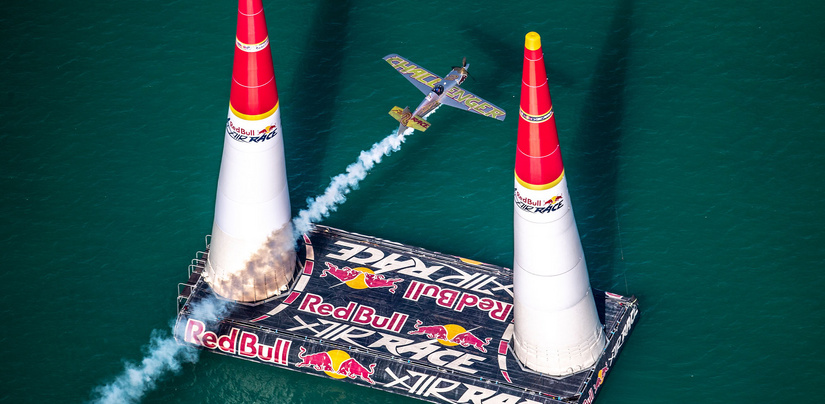
\includegraphics[width=0.8\textwidth]{red-bull-1.jpg}
\end{figure}
"BaffAttack" é um jogo inspirado na corrida de aviões da Red Bull (Red Bull Air Race World Series). O jogo dura 5 minutos e o objetivo é, 
quando o tempo acabar, ter a maior quantidade de pontos. Como será falado à frente, é possível aumentar ou diminuir a duração do jogo.

\begin{center}
\begin{tabular}{|l|}
\hline
\textbf{Plataforma:} PC \\ 
\textbf{Engine:} Godot \\ 
\textbf{Público alvo:} Casual, entusiasta de aviação. Amantes de jogos de precisão. \\ 
\textbf{Controles:} mouse ou teclado \\ 
\hline
\end{tabular}
\end{center}

\section*{Tipo}
Este é um jogo 2D em terceira pessoa top-down, ou seja, com a vista superior do avião com o terreno em baixo.
Foi criado na engine Godot. \cite{godot} \cite{godot-docs}
Uma câmera virtual mantem o avião no centro da tela com o nariz apontado para a frente. Ou seja, quando o avião faz uma curva, o cenário que parece girar na direção contrária. Existe uma suavização na rotação da câmera para que o jogador não tenha uma desorientação espacial, a imagem de fundo também auxilia nisso.

Também seria possível que a câmera seguisse o jogador sem rotacionar, mas, nos testes preliminares, esta opção gerou mais confusão. Quando o avião aponta para baixo, os controles de curva ficam invertidos.